\documentclass{article} % For LaTeX2e
\usepackage{nips15submit_e,times}
\usepackage{hyperref}
\usepackage{url}
\usepackage{graphicx}
%\documentstyle[nips14submit_09,times,art10]{article} % For LaTeX 2.09


\title{ViT Pokemon Classifier}


\author{
Christine Wu\\
Department of Electrical and Computer Engineering\\
University of Washington\\
Seattle, WA 98105 \\
\texttt{wuc29@uw.edu} \\
\And
Pei-Hsuan Lin \\
Department of Electrical and Computer Engineering\\
University of Washington\\
Seattle, WA 98105 \\
\texttt{peihslin@uw.edu} \\
\AND
Zhiwei Zhong \\
Department of Electrical and Computer Engineering\\
University of Washington\\
Seattle, WA 98105 \\
\texttt{zhongz22@uw.edu} \\
\\
}

% The \author macro works with any number of authors. There are two commands
% used to separate the names and addresses of multiple authors: \And and \AND.
%
% Using \And between authors leaves it to \LaTeX{} to determine where to break
% the lines. Using \AND forces a linebreak at that point. So, if \LaTeX{}
% puts 3 of 4 authors names on the first line, and the last on the second
% line, try using \AND instead of \And before the third author name.

\newcommand{\fix}{\marginpar{FIX}}
\newcommand{\new}{\marginpar{NEW}}

\nipsfinalcopy % Uncomment for camera-ready version

\begin{document}


\maketitle

\begin{abstract}
In this report, we present a comprehensive study on the application of Vision Transformers 
(ViTs) for the task of Pokemon classification. While convolutional neural networks (CNNs) 
have been widely used, the ViT has recently emerged as a promising alternative due to the 
self-attention mechanisms. In this project, we implement a ViT model from scratch to explore
the functionality of the ViT. The ViT model captures spatial relationships using 
self-attention mechanisms, enabling it to learn both local and global features. 
In addition, we create a Pokemon Classifier by using a pre-trained ViT model and fine-tuned on
a Pokemon dataset, where the pre-trained model was trained on ImageNet-21k with image resolution 224x224. 
With the help of the pre-train model we obtain about $95.2\%$ accuracy on our Pokemon Classifier. Next, 
we will discuss the performance of our ViT model that we implement from scratch and our Pokemon Classifier.
Finally, we will wrap up with some discussion on future works. \\
Our code can be found here: https://github.com/christinewoo/ee576-cv-vit
\end{abstract}

\section{Related Works}
The field of computer vision has witnessed significant advancements in recent years, 
particularly in the domain of image classification. Traditional approaches for image 
classification heavily relied on convolutional neural networks (CNNs) such as AlexNet 
and VGGNet, which achieved remarkable performance on various benchmark datasets. However, 
the emergence of Vision Transformers (ViTs) has garnered attention as a promising 
alternative for visual recognition tasks.

The concept of Transformers was initially introduced in the field of natural language 
processing (NLP), where it revolutionized machine translation with the Transformer model. 
Transformer was proposed by Vaswani et al(2017)[1]. and it becomes the state-of-the-art 
method in NLP tasks. Inspired by this success, researchers began exploring the application 
of Transformers in computer vision. Cordonnier et al(2020)[2]. showed that images can express 
any convolutional layer by applying the self-attention layer to them. Furthermore, 
Cordonnier et al(2020)[2]. proved that fully-attentional models can combine local behavior 
and global attention based on input content. Dosovitskiy et al(2021)[3]. pioneered the 
concept of Vision Transformers by adapting the Transformer architecture for image 
classification tasks. They demonstrated the effectiveness of ViTs on large-scale image 
datasets like ImageNet, surpassing the performance of CNN-based models.

Since ViTs have shown promise in general image classification tasks, they may be a good 
tool for classifying Pokemon. This report aims to investigate the application of ViTs for 
Pokemon classification and provide insights into the performance and potential of ViTs in 
this specialized domain.

\section{Technical Description, DataLoader}
\label{gen_inst}

% ALGORITHM
Our goal of this project is to learn the ViT architecture, implement from scratch, and
perform image classification on 150 different Pokemon. Below, we describe the individual 
modules in our self-implemented ViT.

\subsection{System Requirements}
We used following Python Packages to facilitate our development: \\
PyTorch [4] \\
PyTorch-Lightning [5] \\
Tkinter [6] \\

In this project, we used two different types of GPUs to train our two models.
We pre-train our self-implemented ViT model on the CIFAR-10 dataset with two NVIDIA GeForce RTX 2080 Ti cards on a Linux machine. \\
We fine-tune on a ImageNet-21k pre-trained model on the Pokemon dataset with a single GeForce RTX 3060 card on a Windows 11 laptop.

\subsection{Algorithm by Step}

1. This module takes in a 2D image with shape $HxWxC$ and flattens the image into 2D patches each with shape $N * (P * P * C)$.
Here $N = {H * W} / {P^2}$, which is the number of patches, and $P$ is the number of pixels for each image patch.

2. We map the flattened patches to a dimension $D$, where $D$ is the constant latent vector size throughout the transformer layers.
These trainable linear projection outputs are the patch embeddings.
We prepend a class token in front of each patch embedding to serve as the image representation that will later be used in the
classification head at the end of the model. Lastly, to retain the positional information of each patch relative to the original image,
a 1D learnable positional embeddings are added.

3. The transformer block takes embedded patches as inputs and passes them a multi-headed self-attention layer (MSA)
followed by a MLP block with two layers and a GELU non-linearity layer. Before the MSA and MLP blocks, a block of Layernorm is added.
Additionally, there are residual connections after every block.

4. The multi-head self-attention module takes in the embedded sequence of tokens and computes the global self-attention.
For each token, it is mapped to $v$, $k$, and $q$ and passed into the scaled dot-product attention head.
The scaled dot product is used to compare the "query" with the "keys" and get scores for the "values."
Each of the scores is in short the relevance between the "query" and each "key".
We reweight the "values" with the obtained scores and take the summation of the reweighted "values".
Lastly, it is concatenated and passed into another linear layer for information flow, which helps to mix the information captured by each head.

5. The classification head is implemented with a MLP consisting of one hidden layer during pre-train.
During the fine-tuning stage, the MLP will consist of one single linear layer.



% Pre-train
\subsection{Pre-trained Model}
For Transformers, and other self-attention-based architectures, the training usually consists of pre-training on 
a large dataset, such as a large text corpus for natural language processing tasks, and then fine-tune on a 
task-specific dataset. In our case, we want to perform image classification, therefore we used the pre-trained weights
released on Hugging Face. The pre-trained weight we have used is "vit-base-patch16-224". It is a ViT model pre-trained
on ImageNet-21k, which consists of 14 millioin images and 21,843 classes. Each of the image has resolution 224x224.
Through this pre-training, the model learns the representation of images that can be used to extract features for the
fine-tune task. The fine-tune training trains a Pokemon classifier by adding a linear layer on top of the pre-trained
ViT encoder for the 150 classes in the Pokemon dataset.

\subsection{Dataloader} % include dataset information

1. CIFAR-10

This dataset contains 60,000 32x32 color images with 10 different classes. The 10 different 
classes represent airplanes, birds, dogs, cars, cats, deers, frogs, horses, ships, and trucks 
and there are 6,000 images of each class. We use 45,000 images as the training dataset, 
5,000 images as the validation dataset, and 10,000 as the test dataset.

The type of our algorithm's input is Datast in PyTorch. We used the build-in function 
tourchvision.datasets.CIFAR10 to download the dataset from the Internet and randomly split 
the entire dataset into the training, validation, and test dataset. 

2. 7,000 Labeled Pokemon

This dataset contains 6837 images with 150 different Pokemon. There are around 25 - 50 
images for each Pokemon. All of the images with the Pokemon in the center. We use 90\% of 
the dataset for training and 10\% of the dataset for testing.

We download the dataset from Kaggle. In the entire dataset, there are many folders that 
are named after one of the Pokemon's names. In each folder, there are several pictures 
of that Pokemon. We use torchvision.dataset.ImageFolder to open this dataset and turn it 
into Dataset in PyTorch. Then we randomly split that dataset into training ad testing 
dataset.


\section{Experimental Results}
\label{headings}
We train our self-implemented ViT model with the CIFAR-10 dataset. It consists of 50,000 RGB training images
and 10,000 test images, both with image resolution 32x32. We use a batch size of 32 and learning rate of 0.0002. The number of 
hidden dimension is set to 128, number of heads is 4, and the number of transformer blocks is 4. We train the model for 30 
epochs. Our Pokemon Classifier was pre-trained on ImageNet-21K and fine-tuned on the Pokemon dataset. We use a 
batch size of 16, learning rate of $5 * 10^{-5}$, and trained for 5 epochs.

We present our experimental results for the self-implemented ViT model and the Pokemon Classifier, respectively:

% \subsection{Experimental Results for Model from Scratch}

\begin{table}[ht]
  \centering
    \begin{tabular}{ c | c | c | c | c  | c | c }
      \hline
      Image Size & Learning Rates & Hidden Dimension & Heads & Number of Blocks & Epoch & Accuracy \\ \hline
      3 x 32 x 32 & 0.0002 & 128 & 4 & 4 & 30 & 62.64\% \\ \hline
      3 x 32 x 32 & 0.001 & 64 & 2 & 6 & 20 & 57.94\% \\ \hline
    \end{tabular}
    \caption{Best Training Results of the Model from Scratch}
  \label{tab:my_label}
\end{table}


% \subsubsection{Experimental Results for Pretrained Model}
\begin{table}[ht]
  \centering
    \begin{tabular}{ c | c | c | c | c  | c }
      \hline
      Item & Epoch 1 & Epoch 2 & Epoch 3 & Epoch 4 & Epoch 5 \\ \hline
      validation loss & 2.62 & 0.9648 & 0.5622 & 0.4275 & 0.371\\ \hline
      validation accuracy & 0.7287  & 0.9124 & 0.9432 & 0.952 & 0.952 \\ \hline
    \end{tabular}
    \caption{Training Results of the Pretrained Model}
  \label{tab:my_label}
\end{table}

\subsection{GUI Development}
We used Python Tkinter package to develop the GUI application of the model.
Our Pokemon Classifier application takes in a RGB image and inference on the best checkpoint.
The predicted result will be the label of the Pokemon class that has the most similar feature 
as the input image.
The application then outputs an image of the corresponding Pokemon label predicted,
along with the name of the Pokemon.
\begin{figure}[h]
\begin{center}
% \framebox[4.0in]{$\;$}
% \fbox{\rule[-.5cm]{0cm}{4cm} \rule[-.5cm]{4cm}{0cm}}
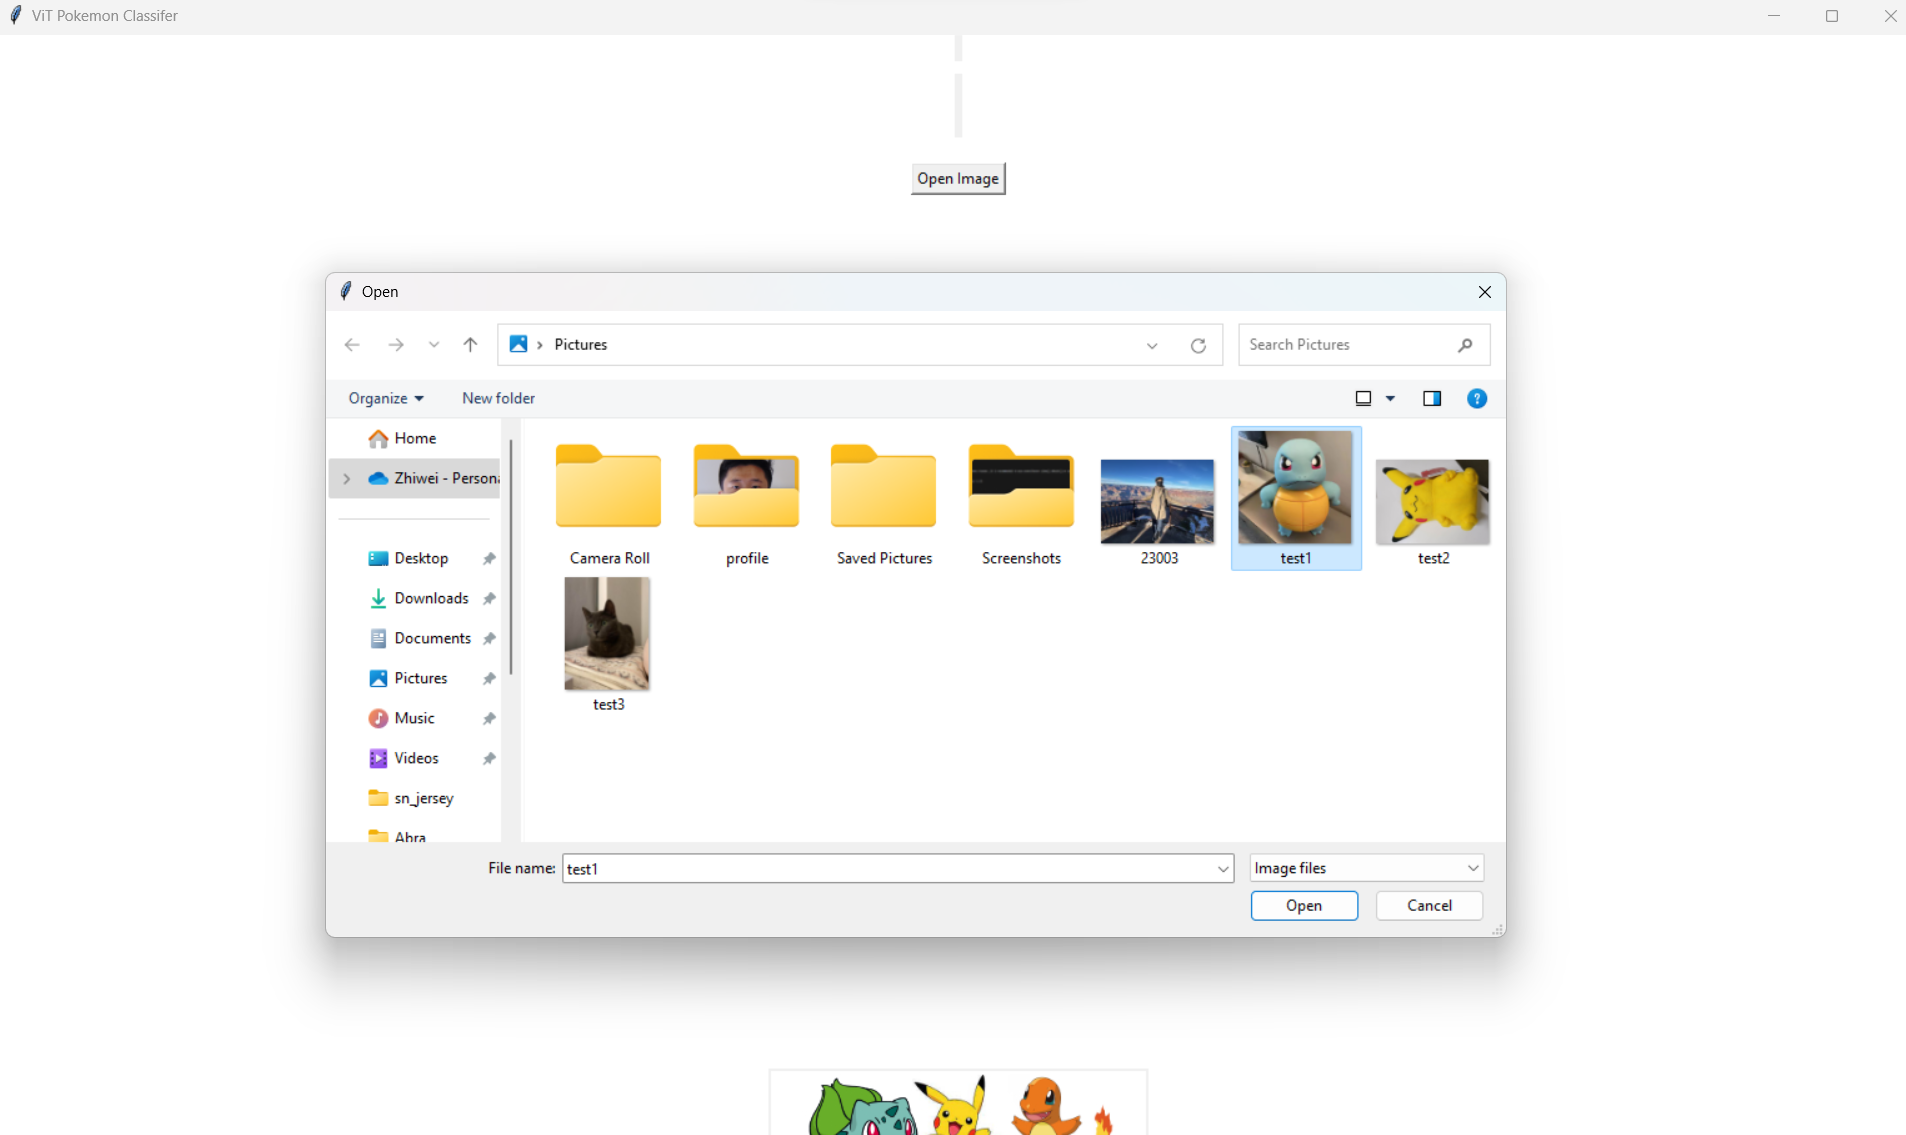
\includegraphics[width=8cm]{gui_process.png}
\end{center}
\caption{Select Input Image to the GUI}
\end{figure}
\begin{figure}[h]
\begin{center}
% \framebox[4.0in]{$\;$}
% \fbox{\rule[-.5cm]{0cm}{4cm} \rule[-.5cm]{4cm}{0cm}}
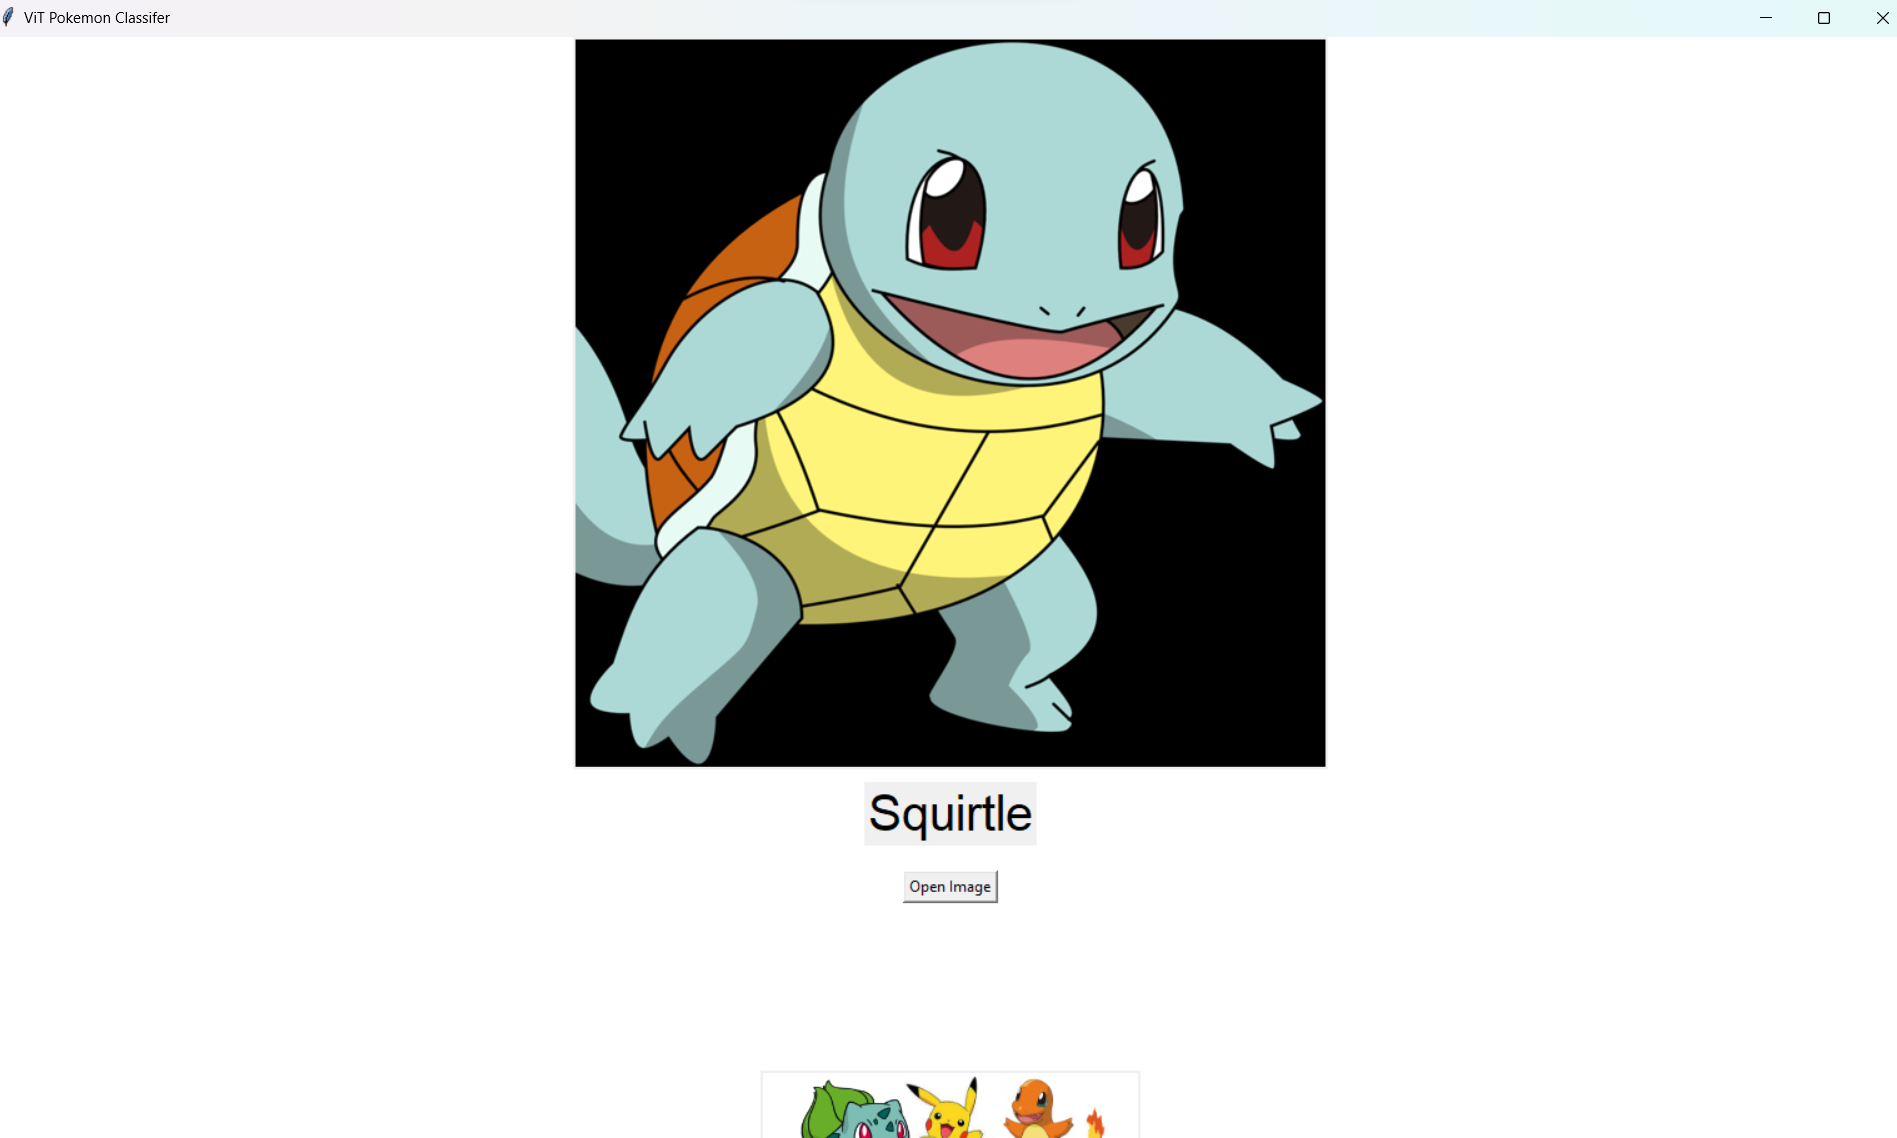
\includegraphics[width=8cm]{gui_result.png}
\end{center}
\caption{GUI Output Result}
\end{figure}


\section{Discussion of Results}
From the results of our self-implemented ViT model, we can see that the model learns better with
a smaller learning rate and deeper hidden layers. Note that the number of hidden dim, the number 
of heads, and the number of blocks should not be too big, since it will quickly increase the complexity
of our model.
After obtaining around 62.64\% for pre-training and 95.2\% on our fine-tuned Pokemon Classifier, 
we can see that ViT indeed works better when it is pre-trained on a general large image classification dataset
before fine-tuning on a smaller task-specific dataset.
Another point to note is that the dataset itself would affect the results of the model. As the 
features or the number of channels of each image increase, the complexity of the model would quickly increase.  


\section{Future Works}
Here are some ideas that we would like to do if we had more time. We would like to inference 
the CIFAR-10 dataset on a CNN model to compare the performance between Transformer based and 
Convolutional based methods. Additionally, to improve our from scratch method, we hope to add 
learning rate scheduler, dropout layers, and replace some for loops for better efficiency.

Lastly, in terms of some modifications on the ViT architecture, one observation is that ViT's 
computational complexity is quadratic to the image size. Meaning, the ViT struggles with high 
resolution images, which is usually the case for most image, such as autonomous driving images 
that are usually 720 x 1280. Another observation is that ViT uses fixed sized tokens, which are 
quite unsuitable in vision tasks such as object detection that needs to extract visual elements 
of various scales.

After some research, we found one paper that tackles some of these ideas, which is the Swin 
Transformer by Microsoft. The Swin Transformer utilizes patch merging to obtain hierarchical 
feature maps, which is similar to the downsampling concept in CNNs. Additionally, the Swin 
Transformer computes window based self-attention instead of global attention to make the 
computational time increase linearly with image resolution. Shifted windows are introduced to 
make sure the correlations between patches within defined windows are exchanged, retaining a 
sense of global attention.

Finally, if we were given more time, we hope to deploy our trained fine-tune Pokemon Classifier 
and simple GUI for people to try!

\subsubsection*{References}

\small{
[1] Vaswani, A., Shazeer, N., Parmar, N., Uszkoreit, J., Jones, L., 
Gomez, A. N., Kaiser, L., \& Polosukhin, I. (2017). Attention is All 
you Need. In {\it arXiv (Cornell University)} (Vol. 30, pp. 5998-6008). 
Cornell University. https://arxiv.org/pdf/1706.03762v5

[2] Cordonnier, J., Loukas, A., \& Jaggi, M. (2020b). On the 
relationship between self-attention and convolutional layers. In {\it International 
Conference on Learning Representations.} https://openreview.net/pdf?id=HJlnC1rKPB

[3] Dosovitskiy, A., Beyer, L., Kolesnikov, A. I., Weissenborn, D., Zhai, X., 
Unterthiner, T., Dehghani, M., Minderer, M., Heigold, G., Gelly, S., Uszkoreit, 
J., \& Houlsby, N. (2021). An Image is Worth 16x16 Words: Transformers for Image 
Recognition at Scale. In {\it International Conference on Learning Representations.}
https://openreview.net/pdf?id=YicbFdNTTy

[4] Pytorch. PyTorch. (n.d.). https://pytorch.org/ 

[5] Pytorch Lightning. Lightning Open Source. (n.d.). https://www.pytorchlightning.ai/index.html 

[6] Tkinter-Python interface to TCL/TK. Python documentation. (n.d.). https://docs.python.org/3/library/tkinter.html 

}


\end{document}